INTRO: 
	- Different ways of realizing them
	- CZ gate


\chapter{Calibrating and Characterizing Controlled Variable Phase Gates}
This chapter details the concepts, calibration and characterization of \glspl{carb}. We start by explaining how they can be seen as extension of standard \glspl{cz}. Next, we demonstrate the implementation of a \glspl{carb} on a physical device and detail their calibration procedure. We perform quantum process tomography for several conditional phases and evaluate the gate fidelity for each case. By exploiting the 3-level readout discussed in Chapter \ref{ch:qutrit_readout}, we then characterize conditional-/dynamic- phase errors and leakage. We compare these values to the ones obtained with a \gls{cz} implemented on the same qubits.  We conclude that the gate performance is sufficient for its envisioned usage in \glspl{vqa} and implement such experiment in Chapter \ref{ch:qaoa}.


\section{Theoretical description} \label{sec:c_arb_theory}
The implementation of a \gls{carb} relies on the same principle as the \gls{cz}, namely the collection of geometric phase on the \oo state\footnote{For the gate discussed in this chapter, $\ket{ij}$ is a short notation for qubit 2 and qubit 3 in states $i$ and $j$ respectively.} due to the interaction of the \oo level and the non-computational \tz level\cite{Strauch2003QuantumQubits, DiCarlo2009DemonstrationProcessor}. To understand this phenomena, we look at the two qutrit interaction Hamiltonian with the rotating wave approximation:

- link to propagator (unitary)
a pair of qubit $A$ and $B$, bringing the \oo state close to the \tz state the interaction Hamiltonian yields the following propagator \cite[p.~87]{Heinsoo2018}: 
\begin{equation}
    \begin{aligned}
U(t)=& e^{-\i t J(|20\rangle\langle 11 |+|  11 \rangle \langle 20|)} \\
=& \mathrm{I}+\left[\cos \left(J t\right)-1\right](|11\rangle\langle 11|+| 20\rangle\langle 20|)-\\
& \i \sin \left(J t\right)(|20\rangle\langle 11|+| 11\rangle\langle 20|)
\end{aligned}
\end{equation}
 where $J$ denotes the coupling strength between the \oo and the \tz state.
 
 The geometric phase acquired by the \oo state during the gate depends on the frequency detuning between the \oo and \tz levels REF HEINSOO. At the qubit parking positions, the detuning is large such that the acquired phase is small (ideally zero). During the gate, we apply a flux pulse to one of the qubits. The pulse shifts the transition frequencies such that the \oo and \tz levels are closer to one another. By varying the amplitude of the flux pulse, we can change the frequency detuning of the interacting levels, and thus the collected phase. The interaction between the two levels also mediates a periodic population exchange between the \oo and \tz states, in addition to the geometric phase of interest. To ensure maximal \oo-state population recovery after the gate, the length of the interaction with the \tz-state has to be a multiple of the population exchange period. The period also depends on the frequency detuning between the \oo and \tz state. 
For a pair of qubit $A$ and $B$, bringing the \oo state close to the \tz state the interaction Hamiltonian yields the following propagator \cite[p.~87]{Heinsoo2018}: 
\begin{equation}
    \begin{aligned}
U(t)=& e^{-\i t J(|20\rangle\langle 11 |+|  11 \rangle \langle 20|)} \\
=& \mathrm{I}+\left[\cos \left(J t\right)-1\right](|11\rangle\langle 11|+| 20\rangle\langle 20|)-\\
& \i \sin \left(J t\right)(|20\rangle\langle 11|+| 11\rangle\langle 20|)
\end{aligned}
\end{equation}
 where $J$ denotes the coupling strength between the \oo and the \tz state. Near resonance, the population is fully swapped back to the \oo state for
 \begin{equation}
     t_{\textrm{gate}} = \frac{2\pi} { \sqrt { \Delta ^ { 2 } + 4 J ^ { 2 } } }
 \end{equation} 
 and the corresponding geometric phase on the \oo state acquired by the closed loop state evolution is 
 \begin{equation} \label{eq:ch4_acquired_cond_phase}
     \phi_{ c } = \pi + \frac{\Delta \cdot t_{\textrm{gate}}}{2} = \pi \cdot \left( 1 + \frac { \Delta } { \sqrt { \Delta ^ { 2 } + 4 J ^ { 2 } } } \right)
 \end{equation}
 with $\Delta = \omega_{\ket{20}} - \omega_{\ket{11}}$ the frequency detuning between the \tz and \oo state. Hence, arbitrary phases can be reached by varying $\Delta$.
 
 Assuming qubit $B$ is fluxed with a pulse of amplitude $a$, $\Delta$ is related to the amplitude through the qubit frequency $\omega _ { | 01 \rangle }(a)$:
 \begin{equation}
\begin{aligned} 
\Delta(a) & = \omega _ { | 20 \rangle } - \omega _ { | 11 | \rangle } \\ 
& = 2 \omega _ { | 10 \rangle } - \alpha _ { A } - \left( \omega _ { | 10 \rangle } + \omega _ { | 01 \rangle }(a) \right) \\ 
& = \omega _ { | 10 \rangle } - \alpha _ { A } - \omega _ { | 01 \rangle }(a) 
\end{aligned}
\end{equation}
Recalling that
\begin{equation}
    \omega_{\ket{01}} \simeq \sqrt{8E_J E_c} - E_c
\end{equation}
and 
\begin{equation}
    E_J = E _ { J , \max } \sqrt { \cos ^ { 2 } \left( \frac { \partial \Phi } { \partial V } a \right) + d ^ { 2 } \sin ^ { 2 } \left( \frac { \partial \Phi} { \partial V } a \right) }
\end{equation}
where $\alpha_A$ denotes the anharmonicity of qubit $A$. 

During the flux pulse, the fluxed qubit is out of its rotating frame and therefore acquires a dynamic phase $\phi_D$:
\begin{equation} \label{eq:carb_dyn_phase}
    \phi_D = \int_0^l{(\omega_t-\omega_{\textrm{park}})\d t}
\end{equation}
where $\omega_{t}$ and $\omega_{\textrm{park}}$ denote the instantaneous qubit frequency during the pulse and the frequency at parking position respectively. 

TODO: read Dicarlo, 
- restate CZ hamiltonian, show that by tuning amplitude and interaction time, we can change the phase to arbitrary value. 
- Chevron pattern --> Need high pop recovery.

Interaction hamiltonian and unitary
Fig: ?

\section{Calibration} 
This section describes the calibration procedure of a \gls{carb} using unipolar, flat-top Gaussian flux pulse on qubit 2 and 3 of the device presented in Appendix \ref{app:setup}. 
For the calibration of the \gls{iir} and \gls{fir} filters, which compensate for the charge accumulation on the bias-tee and the frequency-dependent response of the flux line, we follow the procedure detailed in  \cite{Butscher2018ShapingFiltering}. The filters predistort the flux pulse to achieve the desired pulse shape at the quantum device.

The calibration of the \gls{carb} consists of three measurements, illustrated in Fig. \ref{fig:ch4_calibration_carb}.

First, we prepare the \oo state and perform a two-dimensional sweep of the flux pulse amplitude and length. For each amplitude and length, we measure the \e level population of qubit 2 after the flux pulse using 3-level readout. This results in a chevron pattern shown in the background of the left panel in Fig. \ref{fig:ch4_calibration_carb}a. Brighter areas correspond to high \e level population of qubit 2, indicating the population is fully swapped back from the \f level into the computational subspace. To find the (shortest) pulse lengths resulting in maximal population recovery, we fit for each pulse amplitude the \e level population oscillation to a cosine. We then retrieve the pulse length corresponding to the first maximum of the population oscillation. (SHOULD IT BE PART OF A FIGURE?)

We fit these maximum to the model described in Section \ref{sec:c_arb_theory}, where the free parameters are the flux sensitivity and the coupling strength between the \oo and \tz states. The fit is shown in dashed line in Fig. \ref{fig:ch4_calibration_carb}a.

Next, we measure the conditional phase acquired for different flux pulse amplitudes (see Fig. \ref{fig:ch4_calibration_carb}b). For each amplitude, the length of the pulse is adapted to the value obtained with the chevron measurement to ensure full population recovery.  
To visualize this effect, we overlay the measurement points of Fig. \ref{fig:ch4_calibration_carb}b on Fig. \ref{fig:ch4_calibration_carb}a at the corresponding amplitude and pulse length. The colored flux pulses shown Fig. \ref{fig:ch4_calibration_carb}d correspond to the diamond-shaped data points of respective color in Fig. \ref{fig:ch4_calibration_carb}a and b. The expected conditional phase obtained by \eqref{eq:ch4_acquired_cond_phase} is shown in dashed line. As the flux pulse amplitude tends to zero, the model predicts a conditional phase of 0. Nevertheless, the observed conditional phase saturates at a value of $\sim 0.4$ radians, which corresponds to the phase acquired during the calibration due to the  400\unit{kHz} residual $zz$-coupling between qubit 2 and qubit 3. 

Finally, we measure the dynamic phase the fluxed qubit acquires during to its frequency excursion (see Fig. \ref{fig:ch4_calibration_carb}c). With the approximation that its frequency is constant over the entire pulse at the value given by Eq. \eqref{eq:carb_omega_01_pulsed}, the dynamic phase is computed from Eq. \eqref{eq:carb_dyn_phase} and shown in dashed line. As the dynamic phase is measured between 0 and $2\pi$ but in fact wraps around many times, this measurement requires a high sampling rate to avoid interpolation errors. In Fig. \ref{fig:ch4_calibration_carb}c, only one out of three point is shown for clarity. When used in an algorithm, the dynamic phase is compensated for by applying a virtual Z gate to the fluxed qubit after the flux pulse. 

Due to flux crosstalk between the charge lines, the qubit staying at its parking position also acquires a non-zero dynamic phase. However, the later is not calibrated as flux crosstalk between charge line 1 (3) and qubit 2 is smaller than 2\% (3\%) for the two two-qubit gates considered in this report \cite{Andersen2018SampleB4QP3}.

\begin{figure}
    \centering
    \includegraphics[width=\textwidth]{chapters/carb_gate/figs/ch4_carb_calibration_20200122_174703_with_pulses.png}
    \caption{Three calibration measurements of a \gls{carb} and their pulse schemes. Single qubit $R_x^\pi$, $R_x^{\pi/2}$ and readout pulse are shown in yellow, purple and orange respectively. A dashed pulse indicates the measurement is performed once without and once with the pulse. (a) Qubit 2 \e level population as function of the flux pulse amplitude and length. The inset details the pulse scheme: the \oo state is prepared, the flux pluse is  applied to qubit 3 (black), the two qubits are read out with a multiplexed readout pulse. The scattered points correspond to the amplitudes and lengths used to calibrate the conditional phase (see b). The dashed line corresponds to a fit to a theoretical model. (b) Conditional phase as function of flux pulse amplitude. The amplitude sampling is not uniform to account for the non linearity of the conditional phase. The dashed line indicates the phase prediction of the model. The phase is measured on qubit 2 with a Ramsey experiment, while qubit 3 is fluxed with and without preceding single qubit rotation. The difference between the two measurements yields the conditional phase. (c) Unwraped dynamic phase of qubit 3 as function of amplitude. Only one out of three data point is shown for clarity. The dynamic phase is measured by comparing the qubit phase with and without flux pulse. The dashed line corresponds to the predicted dynamic phase by theory.}
    \label{fig:ch4_calibration_carb}
\end{figure}

The measurement time required for a full \gls{carb} calibration on qubits 2 and 3 amounts to approximately 2h45min: 1h for the chevron, 15min for the conditional phase, and 1h30min for the dynamic phase. The calibration time can be reduced in several ways:
\begin{itemize}
    \item[--] Use the active reset scheme discussed in Section \ref{sec:active_reset}. This scheme allows an increase of the repetition rate by a factor of 5-10 leading to a total measurement time of 20-40 minutes.
    \item[--] Use a non-linear amplitude sampling for the dynamic phase based on the theoretical model. Namely, have an adaptable spacing between amplitudes at which the dynamic phase is calibrated based on whether the model predicts a large or small increase in dynamic phase. This would reduce the number of measurement point for the dynamic phase calibration by a factor of 2, compared to a dense linear spacing.
    \item[--] Rewrite the dynamic phase measurement such that all waveforms are uploaded on the AWGs at once, instead of one at the time. This would reduce communication overhead.
\end{itemize}
Implementing these changes could reduce the calibration time to under 20min per gate. Parallel tune up of two qubit gates has the potential to decrease the calibration time of the device even further. 

In this section, we demonstrated the ability to calibrate a \gls{carb}. The next section details the characterization of the gate after its calibration.

\section{Characterization} 
Randomized benchmarking -- the most common method to characterize two qubit gates -- cannot be performed on the \gls{carb} because it is not part of the Clifford group \cite{Magesan2011ScalableProcesses, Magesan2012CharacterizingBenchmarking}. Hence, we use another common method called quantum process tomography to characterize the \gls{carb}. Next, we perform a fine target phase sweep and characterize conditional and dynamic phase errors as well as leakage outside the computational subspace. Finally, we compare the performance of the \gls{carb} to the \gls{cz} and assess their time stability over a period of 15 hours.

\subsection{Quantum process tomography}
\gls{qpt} is a method providing full description of a quantum process \cite{Chuang1997PrescriptionBox, Poyatos1997CompleteGate}. In brief, it consists of preparing an ensemble of input states $\{\rho_1^\mathrm{in}, ..., \rho_k^\mathrm{in}\}$ spanning the Hilbert space of interest, passing them through the quantum process $\mathcal{E}$ and finally identifying the resultant states  $\{\rho_1^\mathrm{out}, ..., \rho_k^\mathrm{out}\}$ using quantum state tomography \cite{Reed2013EntanglementQubits}. The output states are then
\begin{equation}
    \rho_k^{\mathrm{out}} = \mathcal{E}(\rho_k^\mathrm{in}) = \sum_{m n} \chi_{m n} P_n \rho_k^\mathrm{in} P_m^\dag
\end{equation}
 where $\chi$ is the process matrix and $P$ is the Pauli operator basis for 2 qubits: $\{I, X, -\i Y, Z\}^{\otimes 2}$ \cite{HeinsooDigitalQubits}. The inversion of the above equation yields the desired matrix $\chi$. 
 
Process fidelity $\mathcal{F}$ quantifies the closeness between the measured process matrix $\chi_\mathrm{exp}$ and the target matrix $\chi\mathrm{targ}$ \cite{Schumacher1996SendingChannels}: 
 \begin{equation}
     \mathcal{F} = \mathrm{Tr}(\chi_\mathrm{exp} \chi_\mathrm{targ})
 \end{equation}
This metric indicates how well the channel preserves entanglement.
In the presence of leakage, the tomographic reconstruction of the computational subspace is not a trace-preserving map \cite{Wood2018QuantificationErrors}. Therefore, we use the 3 level readout scheme discussed in Chapter \ref{ch:qutrit_readout} to detect and exclude leakage event from the tomography measurement. We characterize leakage occuring during the gate separately in Section \ref{sec:carb_characterization_phase_errors_leakage}. 
Noise in the measurement can also lead to non-physical\footnote{A physical density matrix is positive semidefinite, Hermitian and trace preserving.} density matrices reconstructions. We use a maximum likelihood algorithm to find physical density matrices which are most likely to have been measured under the assumption of Gaussian noise \cite{BaurRealizingQubits}. 
Finally, we correct for readout errors by multiplying the measured probabilities with the inverse of the readout probability matrix (see Supplementary Material \cite{Bialczak2010QuantumQubits}).

We perform \gls{qpt} for various angles of the \gls{carb}. Two resulting process matrices, $\chi^\pi$ and $\chi^{7\pi/4}$,  for target phases of $\pi$ and $7\pi/4$ respectively are shown in Fig. \ref{fig:carb_characterization_chi_matrices}. The black frame represents the target process matrices while the filled bars correspond to the reconstructed process matrices. We observe an good qualitative agreement between them. In the chosen basis, a process matrix which can be described by a real unitary operator will also be real \cite{Nielsen2000QuantumInformation}. This is the case for $\chi^\pi$, which is described by the real diagonal \gls{cz} unitary. REF TO UNITARY. By contrast, $\chi^{7\pi/4}$ is not described by a real unitary operator and therefore contains an imaginary part. On the diagonal of the real part, the same terms appear as in the $\chi^{\pi}$, but with a different relative contribution. In particular, the $II$ contribution is higher, as adding a phase of $7\pi/4$ (nearly $2\pi$) on the \oo state is closer to an identity operation than adding a phase of $\pi$.

\begin{figure}[ht]
    \centering
    \includegraphics[width=\textwidth]{chapters/carb_gate/figs/ch4_characterization_chi_matrices.png}
    \caption{Real (a, c) and imaginary (b, d) elements of the process matrices $\chi^\pi$ and $\chi^{7\pi/4}$ respectively. The black wire frame corresponds to the target process matrix, while the blue (positive values) and red (negative values) filled bars correspond to the recontructed process matrix from measurements. The process fidelity of for the phase $7\pi/4$ ($\pi$) is 98.3\% (97.3\%).   }
    \label{fig:carb_characterization_chi_matrices}
\end{figure}


In Fig. \ref{fig:carb_characterization_process_fidelity}, we show the process fidelity for 7 phase angles of the \gls{carb}. The maximun (minimum) fidelity is $98.3\%$ ($97.3\%$), for a phase of $7\pi/4$ ($\pi$). The expected fidelity from a master equation simulation including effects of decoherence during the gate is shown in dotted line. It explains about 1 \gls{pp}, and is largest near phases of $\pi$. Thermal population  (0.4\% (1.3\%) at the time of the measurement on qubit 2 (3)) also affects the fidelity of the gate. Nevertheless, evaluating its effect precisely is non trivial: during \gls{qpt} the thermal population is mixed into other states with the tomography preparation pulses. Therefore, we scale the fidelity obtained by simulation by the probability that both qubits are in the ground state before starting the measurement. We suggest that this constitutes an approximate lower bound for the fidelity. This lower bound corresponds to the dashed line in Fig. \ref{fig:carb_characterization_process_fidelity}. 

\begin{figure}[ht]
    \centering
    \includegraphics[width=\textwidth]{chapters/carb_gate/figs/ch4_characterization_tomo_all_angles_20200124_162200.png}
    \caption{Process fidelity as function of conditional phase angle of the \gls{carb}. Measurements are shown in scattered points.  Master equation simulation including effects of decoherence in dotted line. The dashed line corresponds to the fidelity of the simulation scaled by the probability of starting the measurement in the ground state. }
    \label{fig:carb_characterization_process_fidelity}
\end{figure}

\subsection{Phases errors and leakage} \label{sec:carb_characterization_phase_errors_leakage}
Although \gls{qpt} allows to get full information of the quantum process, it also has several downsides. It is a time consuming measurement and does not provide a direct and intuitive explanation about where errors come from. Finally, it does not include information about leakage. 

A natural way to test the gate before its usage in an algorithm is to attempt to achieve a target conditional phase and assess how close the measured conditional phase is from the target. When using 3 level readout, this measurement also characterizes the \f level population of the qubit leaving the computational subspace (in this case, qubit 2) for each target angle. Similarly, we assess how well we are able to predict the dynamic phase the fluxed qubit acquires.

We perform such sweep over target conditional phase in the range $[0, 2\pi[$ and present the results in Fig. \ref{fig:carb_characterization_phase_errors_leakage}. For all target conditional phases, the error both on dynamic and conditional phase stays within $\pm 4.5$ deg. ($\pm 1.5 \%$ of a full circle). We argue that these errors will not be the limiting factor when used in algorithms. For instance, in the same amount of time ($50-150 \unit{ns}$), the 400\unit{kHz} residual $zz$-coupling would progressively induce a phase error of 7-20 degrees on the \oo state.   NOTE ON TRANSLATION TO GATE INFIDELITY ?

Leakage outside of the computational subspace shows an angular dependency. It is minimum ($\sim 10^{-3}$) for conditional phases far from 180 deg., namely when the gate is very short and the \oo and \tz states are strongly off resonant. By contrast, we observe leakage of up to $2\%$ when the \oo and \tz states are near resonance. For a fixed probability of the excitation to stay in the \tz state, the total population remaining in the \tz state will be maximal at resonance, where the population exchange between the two states is maximal. The dominant contribution to leakage is are the short timescale distortions of the flux pulse \cite{Rol2019Time-domainProcessor} which are not perfectly compensated by the \gls{fir} filters \cite{Butscher2018ShapingFiltering}.  Leakage of qubit 3, which does not go into the \f level during the pulse, is on the order of $10^{-4}$ for all target conditional phases.

\begin{figure}[ht]
    \centering
    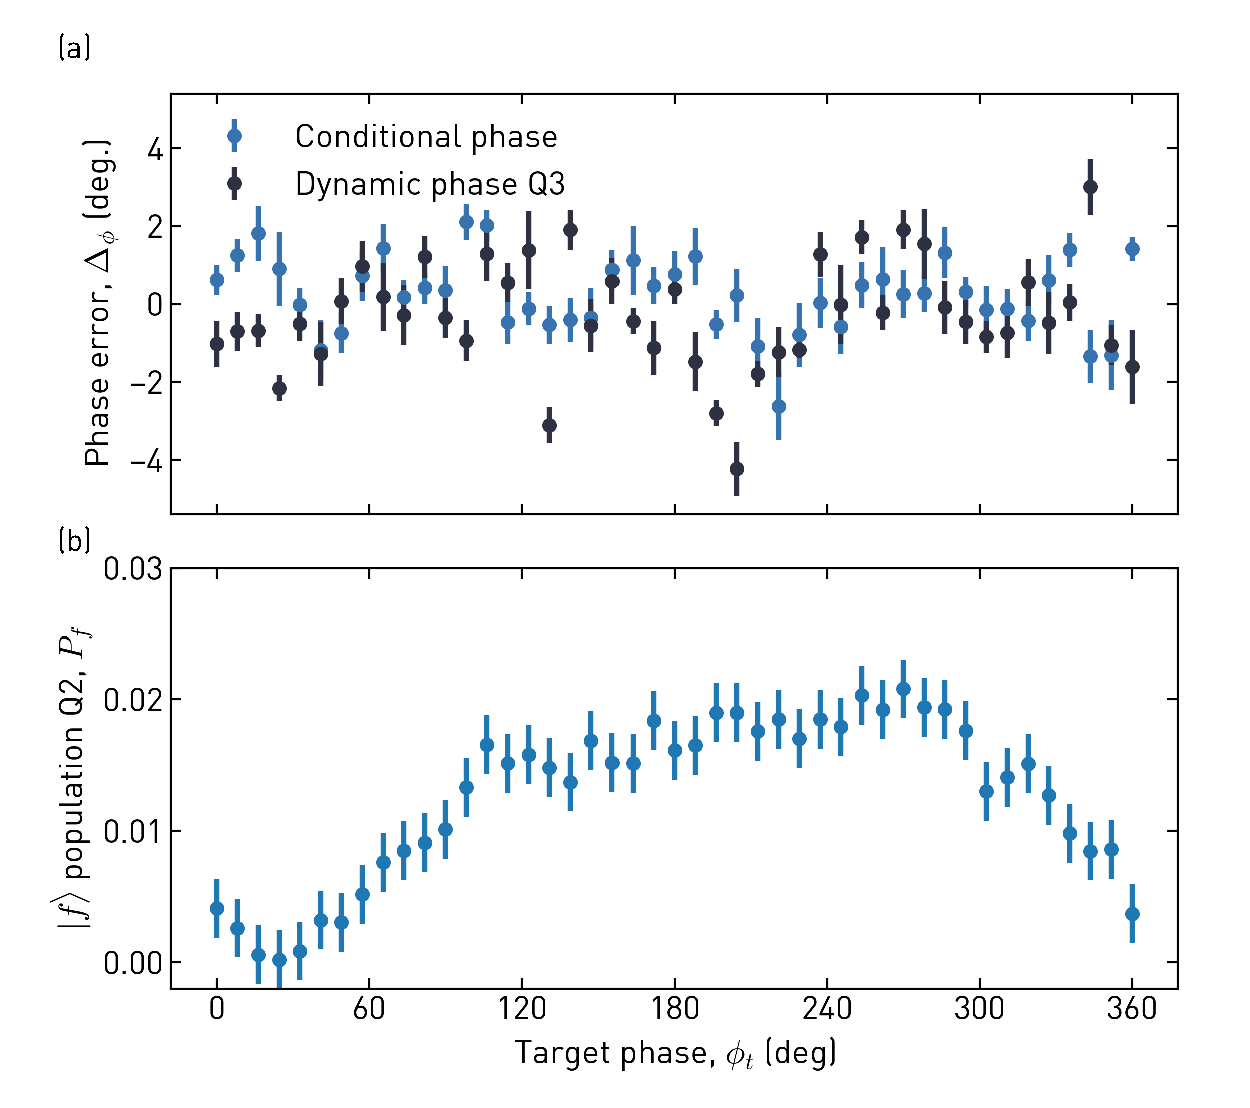
\includegraphics[width=\textwidth]{chapters/carb_gate/figs/ch4_characterization_phase_error_and_leakage_20200126_094856.png}
    \caption{Characterization of phase errors and leakage as function of target conditional phase right after calibration. Each point is averaged over 40000 single shots. Conditional and dynamic phase errors (top panel) are within $\pm 4.5$ deg. We use 3 level readout to characterize leakage (bottom panel). shows an angular dependency}
    \label{fig:carb_characterization_phase_errors_leakage}
\end{figure}

\subsection{Comparison between \glspl{carb} and \glspl{cz}}
As final characterization procedure, we compare the \gls{carb} and \gls{cz} (implemented on the same qubits) in terms of phase errors, leakage and time drift. We calibrate both gates and repeat the measurement described in Section \ref{sec:carb_characterization_phase_errors_leakage}. For the \gls{cz}, we target $N$ times a conditional phase of 180 deg.  For the \gls{carb}, we sweep with $N$ points the range of target phases from 0 to 360 deg. These measurements are repeated up to 15 hours after calibration. The distributions of deviations from target phases and leakage are presented in shaded in Fig. \ref{fig:carb_characterization_drift}.

Both gates exhibit similar range of conditional phase errors. We conclude that extending the \gls{cz} gate to a \gls{carb} gate does not affect how well we are able to prepare a target conditional phase. Note that the \gls{cz} shows a consistent offset of approximately 1 deg. with respect to its target conditional phase. This originates from the fact that the gate is calibrated with a single point measurement, which in this case was on the lower end of the distribution. 

The \gls{carb} results into wider distribution of dynamic phase errors, with an average standard deviation of 1.25 deg. versus 0.85 deg. for the \gls{cz}. This indicates it is indeed harder to calibrate the dynamic phase for many flux pulse amplitudes and lengths simultaneously compared to calibrating only one.

The qubit 2 leakage dynamics are consistant with the discussion in Section \ref{sec:carb_characterization_phase_errors_leakage}: the \gls{cz} experiences an average leakage of approximately 2\% since the \oo and \tz levels are on resonance. By contrast, the \gls{carb} experiences an average leakage of 1.4\% as several conditional phases result in low leakage. Its worse case leakage, however, is comparable to the one of the \gls{cz}. 

The time stability of both gates suggests they will provide stable performance in algorithms for up to 15 hours after calibration.

The gates also differ in their average lengths. This effect is best visualized in Fig. \ref{fig:ch4_calibration_carb}a. While the \gls{cz} has a flux pulse length of $107\unit{ns}$, the \gls{carb} has a varying flux pulse length. Average over all conditional phases, the flux pulse length is $84\unit{ns}$ long or $\sim 20\%$ shorter than for a conditional phase of 180 deg. For both implementations, we add a $10\unit{ns}$ ($15\unit{ns}$) buffer at the stard (end) to avoid overlap of other gates with the rising and falling edges of the flux pulse.

\begin{figure}[ht]
    \centering
    \includegraphics[width=\textwidth]{chapters/carb_gate/figs/ch4_characterization_drift_20200124_175455.png}
    \caption{Comparison between the \gls{cz} (green) and \gls{carb} (blue) in terms of phase errors and leakage.}
    \label{fig:carb_characterization_drift}
\end{figure}

\section{Conclusion}
TODO: write summary of chapter

simple extension of cz

many point calibration

process tomo 97-98

gate/phase errors small

leakage avg 1.4

shorter

Use as building block in QAOA

